% Figs. 7 and 8 belong to Section IV; model.tex inputs this file at the end of III-C,
% so the two figures pair at the top of the next page
\begin{figure}[t]
\centering
\providecommand{\stagefont}{\ttfamily\tiny}
% the sliced policy over the states of fig:policy-ordinary; steps and counter
% values from models.v lemmas sliced_states_no_dI / _with_dI
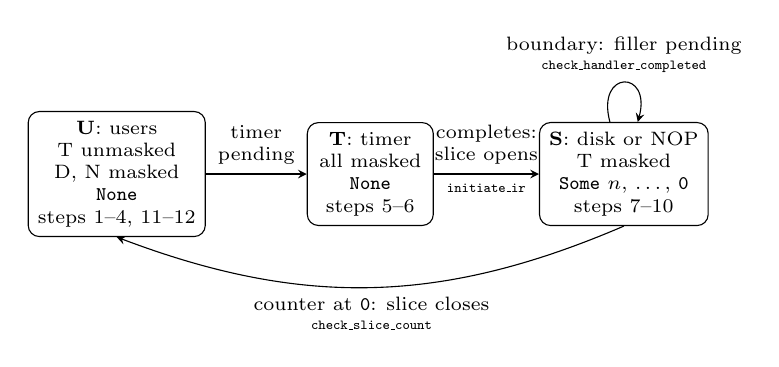
\begin{tikzpicture}[font=\scriptsize, >=stealth,
  ph/.style={draw, rounded corners, align=center, minimum width=1.6cm,
    minimum height=1.1cm, inner sep=3.5pt},
  note/.style={align=center, font=\scriptsize},
  secret/.style={->, line width=1.2pt},
  stage/.style={font=\stagefont}]
\node[ph] (u) at (0,0)   {\textbf{U}: users\\T unmasked\\D, N masked\\\texttt{None}\\steps 1--4, 11--12};
\node[ph] (t) at (3.22,0) {\textbf{T}: timer\\all masked\\\texttt{None}\\steps 5--6};
\node[ph] (s) at (6.44,0) {\textbf{S}: disk or NOP\\T masked\\\texttt{Some} $n$, \ldots, \texttt{0}\\steps 7--10};
\draw[->] (u) -- node[above, note]{timer\\pending} (t);
\draw[->] (t) -- node[above, note]{completes:\\slice opens} node[below, stage]{initiate\_ir} (s);
\draw[->] (s) to[loop above, looseness=5] node[above, note]{boundary: filler pending\\[-1pt]{\stagefont check\_handler\_completed}} (s);
\draw[->] (s.south) to[bend left=22] node[below, note]{counter at \texttt{0}: slice closes\\[-1pt]{\stagefont check\_slice\_count}} (u.south);
\end{tikzpicture}
\caption{The sliced policy over the states of \cref{fig:policy-ordinary}, with the slice
  counter in each state. No arrow is bold: S is entered only when the timer handler
  completes, and left only when the counter, loaded with
  $\mathit{runs}\cdot\mathit{runtime}$, reaches zero. Inside S the disk handler, if
  pending, takes a run the NOP handler would otherwise fill; that choice is all the
  secret decides. Each arrow is labelled with the stage of the service policy that
  takes it. Steps are those of both runs in \cref{fig:run-sliced}.}
\label{fig:phases}
\end{figure}
\begin{figure}[t]
\centering
% runs: models.v Section 11 traces; state rows: lemmas sliced_states_no_dI/_with_dI
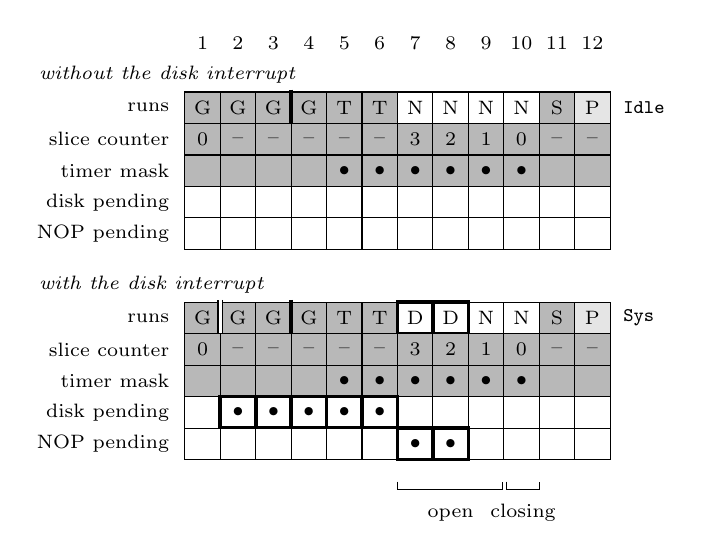
\begin{tikzpicture}[font=\scriptsize,
  cell/.style={draw, minimum width=0.45cm, minimum height=0.4cm, inner sep=0pt},
  pub/.style={cell, fill=black!28}, priv/.style={cell, fill=white},
  cG/.style={pub}, cT/.style={pub}, cS/.style={pub}, cP/.style={cell, fill=black!10},
  cD/.style={priv}, cN/.style={priv},
  head/.style={anchor=west, font=\scriptsize\itshape},
  diff/.style={draw, line width=1.3pt, minimum width=0.45cm, minimum height=0.4cm},
  irq/.style={line width=1.6pt},
  dsk/.style={double, double distance=1.1pt, line width=0.55pt}]
\foreach \i in {1,...,12} \node at (0.45*\i, 0.4) {\i};
% without the disk interrupt
\node[head] at (-1.75,0.00) {without the disk interrupt};
\node[anchor=east] at (0.15,-0.42) {runs};
\foreach \c [count=\i] in {G,G,G,G,T,T,N,N,N,N,S,P} \node[c\c] at (0.45*\i,-0.42) {\c};
\draw[irq] (1.575,-0.19) -- (1.575,-0.65);
\node[anchor=west] at (5.67,-0.42) {\texttt{Idle}};
\node[anchor=east] at (0.15,-0.82) {slice counter};
\foreach \c [count=\i] in {0,{--},{--},{--},{--},{--},3,2,1,0,{--},{--}} \node[pub] at (0.45*\i,-0.82) {\c};
\node[anchor=east] at (0.15,-1.22) {timer mask};
\foreach \c [count=\i] in {{},{},{},{},{$\bullet$},{$\bullet$},{$\bullet$},{$\bullet$},{$\bullet$},{$\bullet$},{},{}} \node[pub] at (0.45*\i,-1.22) {\c};
\node[anchor=east] at (0.15,-1.62) {disk pending};
\foreach \c [count=\i] in {{},{},{},{},{},{},{},{},{},{},{},{}} \node[priv] at (0.45*\i,-1.62) {\c};
\node[anchor=east] at (0.15,-2.02) {NOP pending};
\foreach \c [count=\i] in {{},{},{},{},{},{},{},{},{},{},{},{}} \node[priv] at (0.45*\i,-2.02) {\c};
% with the disk interrupt
\node[head] at (-1.75,-2.67) {with the disk interrupt};
\node[anchor=east] at (0.15,-3.09) {runs};
\foreach \c [count=\i] in {G,G,G,G,T,T,D,D,N,N,S,P} \node[c\c] at (0.45*\i,-3.09) {\c};
\foreach \i in {7,8} \node[diff] at (0.45*\i,-3.09) {};
\draw[irq] (1.575,-2.86) -- (1.575,-3.32);
\draw[dsk] (0.675,-2.86) -- (0.675,-3.32);
\node[anchor=west] at (5.67,-3.09) {\texttt{Sys}};
\node[anchor=east] at (0.15,-3.49) {slice counter};
\foreach \c [count=\i] in {0,{--},{--},{--},{--},{--},3,2,1,0,{--},{--}} \node[pub] at (0.45*\i,-3.49) {\c};
\node[anchor=east] at (0.15,-3.89) {timer mask};
\foreach \c [count=\i] in {{},{},{},{},{$\bullet$},{$\bullet$},{$\bullet$},{$\bullet$},{$\bullet$},{$\bullet$},{},{}} \node[pub] at (0.45*\i,-3.89) {\c};
\node[anchor=east] at (0.15,-4.29) {disk pending};
\foreach \c [count=\i] in {{},{$\bullet$},{$\bullet$},{$\bullet$},{$\bullet$},{$\bullet$},{},{},{},{},{},{}} \node[priv] at (0.45*\i,-4.29) {\c};
\foreach \i in {2,3,4,5,6} \node[diff] at (0.45*\i,-4.29) {};
\node[anchor=east] at (0.15,-4.69) {NOP pending};
\foreach \c [count=\i] in {{},{},{},{},{},{},{$\bullet$},{$\bullet$},{},{},{},{}} \node[priv] at (0.45*\i,-4.69) {\c};
\foreach \i in {7,8} \node[diff] at (0.45*\i,-4.69) {};
\draw (2.925,-5.17) -- (2.925,-5.27) -- (4.255,-5.27) -- (4.255,-5.17);
\node[anchor=north, text height=1.5ex, text depth=.25ex] at (3.600,-5.27) {open};
\draw (4.305,-5.17) -- (4.305,-5.27) -- (4.725,-5.27) -- (4.725,-5.17);
\node[anchor=north, text height=1.5ex, text depth=.25ex] at (4.520,-5.27) {closing};
\end{tikzpicture}
\caption{The sliced policy on the same inputs, laid out as \cref{fig:run-ordinary}; N: NOP handler. The disk and NOP masks are set between all steps and are not shown. The framed cells, where the runs differ, are all private: the disk pending bit until the slice opens, then which handler fills the first run and the NOP pending bit. On the right, the private user's output at step 12; the braces mark the slice, its last step being the closing one (\cref{fig:phases}).}
\label{fig:run-sliced}
\end{figure}
